\documentclass{article}
\usepackage[utf8]{inputenc}
\usepackage{graphicx}
\usepackage{MnSymbol}

\title{\textbf{Van Emde Boas tree}}
\author{Alex Falzone }
\date{2020/2021}

\begin{document}

\maketitle
\section{Introduzione}
\section{Struttura albero}
\section{Operazioni vEB}
\subsection{Minimo e Massimo}
\subsection{Successore e Predecessore}
\subsection{Inserimento}
\subsection{Cancellazione}
\newpage

\begin{flushleft}
\huge \textbf{1. Introduzione}
\newline
\newline
\normalsize
    
    Creato nel 1975 dall'informatico Peter van Emde Boas e successivamente affinato da van Emde Boas, Kaas e Zijlstra.\\
    Questo albero supporta le operazioni di inserimento, cancellazione, successore, predecessore, massimo, minimo e ricerca nel tempo O(lg(lg(u))).
    Un albero di van Emde Boas (abbreviato anche come vEB) deve avere delle caratteristiche ben precise:
    \begin{itemize}
        \item Un attributo \textbf{u} che rappresenta la dimensione dell'albero
        \item Un attributo \textbf{min} che memorizza l'elemento minimo.
        \item Un attributo \textbf{max} che memorizza l'elemento massimo.
        \item Un array \textbf{cluster} di dimensione $\sqrt{u}$
        \item Un array \textbf{summary}[0 $\dots$ $\sqrt{u}$ - 1], dove summary[i] contiene 1 se e soltanto se l'i-esimo cluster[i$\sqrt{u}$ $\dots$ (i + 1)$\sqrt{u}$ - 1] contiene un 1.
    \end{itemize}
    Inoltre non sono ammesse chiavi duplicate.\\
\end{flushleft}

\begin{figure}[h!]
    \begin{center}
    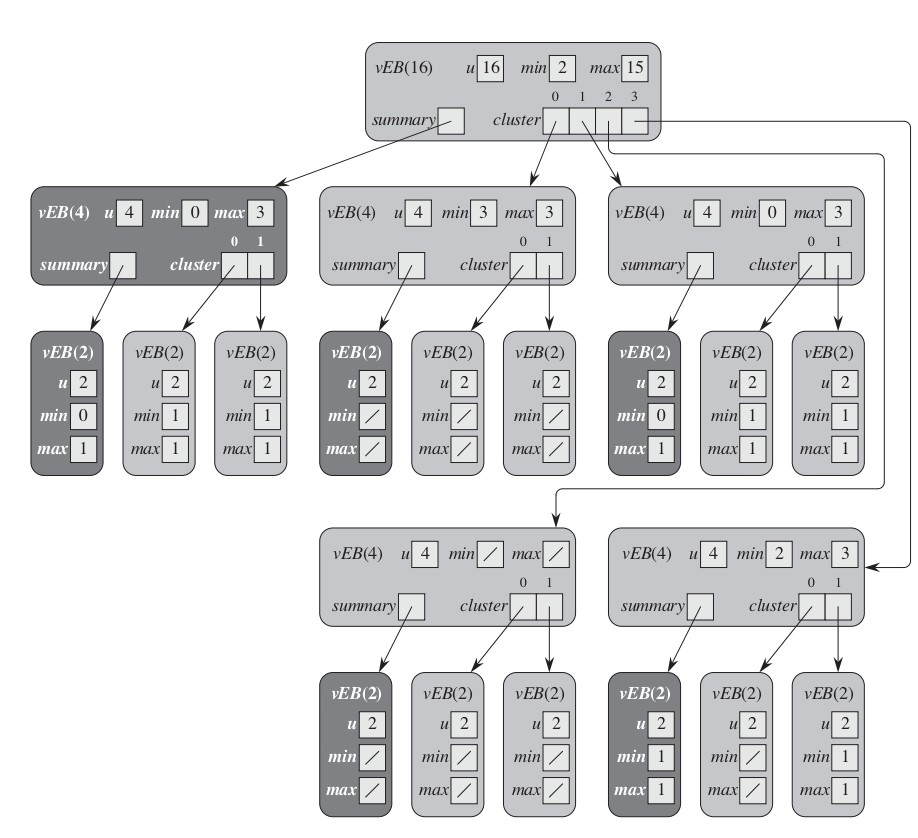
\includegraphics[width=9cm]{vEB.jpg}\\
    \caption{Esempio albero di van Emde Boas (immagine tratta da "Introduction to Algorithm")}
    \end{center}
\end{figure}


\newpage
\begin{flushleft}
\huge \textbf{2. Struttura dell'albero}
\newline
\newline
\normalsize
    
    Indichiamo con $\sqrt[\downarrow]{u}$ la radice quadrata \textbf{inferiore}, ovvero $2^{\lfloor lg(u) / 2 \rfloor}$.\\
    Mentre con $\sqrt[\uparrow]{u}$ la radice \textbf{superiore}, ovvero $2^{\lceil lg(u) / 2 \rceil}$.\\
    Denotiamo con vEB(u) un albero vEB con dimensione dell'universo pari a \textbf{u} e, a meno che u non sia uguale alla dimensione base 2, l'attributo summary punta a un albero vEB($\sqrt[\uparrow]{u}$) e l'array cluster[ 0 $\dots$ $\sqrt[\uparrow]{u}$ - 1] punta ai $\sqrt[\uparrow]{u}$ alberi vEB($\sqrt[\downarrow]{u}$).\\
    Successivamente è necessario stabilire come accedere sia al numero di cluster di un determinato valore(x), sia alla posizione del valore(x) all'interno del cluster; Esso avviene usando rispettivamente:\\
    \begin{equation}
        high(x) = \lfloor x / \sqrt[\downarrow]{u} \rfloor
    \end{equation}
    \begin{equation}
        low(x) = x mod \sqrt[\downarrow]{u}
    \end{equation}
    \begin{equation}
        index(x, y) = (x\sqrt[\downarrow]{u}) + y
    \end{equation}
    \\
    Dove index rappresenta il numero(x) e la posizione(y) del cluster. 

    Inoltre è importante fissare una ricorrenza che tornerà  utile nei costi delle singole operazioni.
    \begin{equation}
        T(u) \leq T(\sqrt[\uparrow]{u}) + O(1)
    \end{equation}
    Ponendo $m = lg (u)$ abbiamo:
        \begin{center}
            $T(2^m) \leq T(2^{\lceil m/2 \rceil} +O(1)$
        \end{center}
    Poiché $\lceil$ m/2 $\rceil$ $\leq 2m/3$ per ogni $m \ge 2$, si ha
        \begin{center}
            $T(2^m) \leq T(2^{2m/3} + O(1)$
        \end{center}
    Ponendo S(m) = T($2^m$), riscriviamo l'occorrenza come
        \begin{center}
            $S(m) \leq S(2m/3) + O(1)$
        \end{center}
    Grazie al secondo caso del teorema master la ricorrenza ha soluzione S(m) = O(lg m).\\
    Dunque abbiamo T(u) = T($2^m$) = S(m) = O(lg m) = O(lg lg u)
\end{flushleft}

\newpage
\begin{flushleft}
\huge \textbf{3. Operazioni}
\newline
\newline
\normalsize

        \subsubsection{Minimo e massimo}
            MINIMO(V)
            \begin{enumerate}
                \item \textbf{return} V.min
            \end{enumerate}

            MASSIMO(V)
            \begin{enumerate}
                \item \textbf{return} V.max
            \end{enumerate}
            
            Poiché il massimo e il minimo sono memorizzati negli attribuiti \textbf{min} e \textbf{max} essi richiedono tempo costante, ovvero O(1).
\end{flushleft}        
\subsubsection{Successore e Predecessore}
            ~\\SUCCESSORE(V, key)
            \begin{enumerate}
                \item \textbf{if} V.universe == 2
                \item \hspace{10pt} \textbf{if} key == 0 and $key < V.min$
                \item \hspace{30pt} \textbf{return} 1
                \item \hspace{10pt} \textbf{else return} NIL
                \item \textbf{else if} $V.min \neq NIL$ and $ key < V.min$ 
                \item \hspace{10pt} \textbf{return} V.min
                \item \textbf{else} max-low = MASSIMO(V.cluster[high(key)])
                \item \hspace{10pt} \textbf{if} $max-low \neq NIL$ and $low(key) < max-low$
                \item \hspace{30pt} offset = SUCCESSORE(V.cluster[high(key)], low(key))
                \item \hspace{30pt} \textbf{return} index(high(key), offset)
                \item \hspace{10pt} \textbf{else} succ-cluster = SUCCESSORE(V.summary, high(key))
                \item \hspace{30pt} \textbf{if} succ-cluster == NIL
                \item \hspace{50pt} \textbf{return} NIL
                \item \hspace{30pt} \textbf{else} offset = MINIMO(V.cluster[succ-cluster])
                \item \hspace{50pt} \textbf{return} index(succ-cluster, offset)
            \end{enumerate}
            
\begin{flushleft}

            ~\\Iniziamo dal caso base, in cui la dimensione dell'albero è pari a 2.
            In questo caso se key è uguale a 0 e 1, ovvero il nostro ipotetico successore, si trova nel medesimo cluster ritorniamo quest'ultimo. Altrimenti non sarà presente nessun successore e ritorniamo NIL.\\
            Alla riga 5 verifichiamo se esiste il minimo e se la key è minore di quest'ultimo, in caso affermativo la riga 6 restituisce il minimo.\\
            Se ci troviamo alla riga 7 sappiamo che non ci troviamo in un caso base e che key è maggiore del minimo. In questo caso settiamo max-low al massimo valore del cluster di key e (alla riga 8) verifichiamo che il cluster di key abbia qualche elemento maggiore di key stesso, infatti in caso di esito positivo sappiamo che il successore di key si trova da qualche parte nel cluster di key. Se il successore di key si trova all'interno del cluster di key, la riga 9 determina dove si trova e la riga 10 restituisce il successore.\\
            Se arriviamo alla riga 11 allora il cluster di key non ha nessun elemento maggiore di key e dobbiamo cercarlo in cluster successivi. Assegniamo a succ-cluster il cluster successivo di key e se esso è diverso da NIL troviamo il minimo valore del cluster successivo a key (riga 14) e lo restituiamo (riga 15), altrimenti torniamo NIL (riga 13).\\
            La ricorrenza (4) caratterizza il tempo di esecuzione di SUCCESSOR, infatti la procedura chiama se stessa alla riga 9 (su un albero con dimensione \textbf{u} pari a $\sqrt[\downarrow]{u}$ ) o alla riga 11(su un albero con dimensione \textbf{u} pari a $\sqrt[\uparrow]{u}$ ). Quindi controllerà al più un albero vEB con dimensione dell'universo pari $\sqrt[\uparrow]{u}$. Le procedure MINIMO e MASSIMO richiedono tempo O(1), quindi SUCCESSOR viene eseguita nel tempo O(lg(lg(u))) nel caso peggiore.\\     
            
\end{flushleft}        

\begin{flushleft}
            ~\\La procedura PREDECESSORE è simmetrica alla procedura SUCCESSORE, ma con un caso aggiuntivo.\\
            ~\\PREDECESSORE(V, key)
            \begin{enumerate}
                \item \textbf{if} V.universe == 2
                \item \hspace{10pt} \textbf{if} key == 1 and $key > V.max$
                \item \hspace{30pt} \textbf{return} 0
                \item \hspace{10pt} \textbf{else return} NIL
                \item \textbf{else if} $V.max \neq NIL$ and $ key > V.max$ 
                \item \hspace{10pt} \textbf{return} V.max
                \item \textbf{else} min-low = MINIMO(V.cluster[high(key)])
                \item \hspace{10pt} \textbf{if} $min-low \neq NIL$ and $low(key) > min-low$
                \item \hspace{30pt} offset = PREDECESSORE(V.cluster[high(key)], low(key))
                \item \hspace{30pt} \textbf{return} index(high(key), offset)
                \item \hspace{10pt} \textbf{else} pred-cluster = PREDECESSORE(V.summary, high(key))
                \item \hspace{30pt} \textbf{if} pred-cluster == NIL
                \item \hspace{50pt} \textbf{if} $V.min \neq NIL$ and $key > V.min$
                \item \hspace{70pt} \textbf{return} V.min
                \item \hspace{50pt} \textbf{else return} NIL
                \item \hspace{30pt} \textbf{else} offset = MINIMO(V.cluster[succ-cluster])
                \item \hspace{50pt} \textbf{return} index(succ-cluster, offset)
            \end{enumerate}
            
            ~\\Il caso aggiuntivo (alle righe 13-14) si verifica quando il predecessore di key, se esiste, non si trova nel cluster di key. Quindi se il predecessore di key è il valore minimo nell'albero vEB V, allora il predecessore non si trova in alcun cluster.\\
            Questo caso extra non influisce sul tempo di esecuzione dell'algoritmo, di conseguenza il costo sarà uguale a quello di SUCCESSOR, ovvero O(lg lg u).\\
\end{flushleft}        

\begin{flushleft}            
        \subsubsection{INSERIMENTO}
            ~\\Empty-Insert(V, key)
            \begin{enumerate}
                \item V.min = key
                \item V.max = key
            \end{enumerate}
            Questa funzione ci tornerà utile in INSERIMENTO, per cercare di smaltire il codice.\\
        
            ~\\INSERIMENTO(V, key)
            \begin{enumerate}
                \item \textbf{if} V.min == NIL
                \item \hspace{20pt} Empty-Insert(V, key)
                \item \textbf{else if} $x < V.min$
                \item \hspace{20pt} scambia key con V.min
                \item \hspace{20pt} \textbf{if} $V.universe > 2$
                \item \hspace{40pt} \textbf{if} MINIMO(V.cluster[high(key)]) == NIL
                \item \hspace{60pt} INSERIMENTO(V.summary, high(key))
                \item \hspace{60pt} Empty-Insert(V.cluster[high(key)], low(key))
                \item \hspace{40pt} \textbf{else} INSERIMENTO(V.cluster[high(key)], low(key))
                \item \hspace{20pt} \textbf{if} $key > V.max$
                \item \hspace{40pt} V.max = key
            \end{enumerate}
                
                
                
            ~\\Innanzitutto è necessario verificare se l'albero è vuoto, se lo è settiamo min e max a key(riga 1-2).\\
            Successivamente alla riga 3 verifichiamo se key è minore del valore minimo, in tal caso scambiamo min e key. Di conseguenza la nostra key originale diverrà il minimo e il nostro minimo originale diverrà key.\\
            Alla riga 5 se l'albero non si trova nel caso base allora dobbiamo determinare se il cluster dove andrà key è vuoto (riga 6), se lo è, inseriamo il numero di cluster di key nel summary, creiamo un nuovo cluster e inseriamo key come min e max (riga 7-8).\\
            Se invece il cluster non è vuoto inseriamo key nel cluster corrispondente (riga 9).\\
            Le righe 10-11 hanno il compito di aggiornare il campo max se e solo se esso è minore di key.\\
            Possiamo notare come la ricorrenza (4) caratterizzi anche questo algoritmo, infatti viene eseguita la chiamata ricorsiva o nella riga 8 (su un albero vEB con dimensione dell'universo $\sqrt[\uparrow]{u}$) o nella riga 12 (su un albero vEB con dimensione dell'universo $\sqrt[\downarrow]{u}$). La parte restante dell'algoritmo richiede tempo O(1), di conseguenza applicando la ricorrenza (4) abbiamo che il tempo di esecuzione di questo algoritmo è pari a O(lg(lg(u))).
            
\end{flushleft}        
\begin{flushleft}            
        \subsubsection{Cancellazione}
            ~\\CANCELLAZI0NE(V, key)
            \begin{enumerate}
                \item \textbf{if} V.min == V.max
                \item \hspace{10pt} V.min = NIL
                \item \hspace{10pt} V.max = NIL
                \item \textbf{else if} V.universe == 2
                \item \hspace{10pt} \textbf{if} key == 0
                \item \hspace{20pt} V.min = 1
                \item \hspace{10pt} \textbf{else} V.min = 0
                \item \hspace{10pt} V.max = V.min
                \item \textbf{else if} key == V.min
                \item \hspace{40pt} first-cluster = MINIMO(V.summary)
                \item \hspace{40pt} x = index(first-cluster, MINIMO(V.cluster[first-cluster])
                \item \hspace{40pt} V.min = key
                \item \hspace{20pt} CANCELLAZIONE(V.cluster[high(key)], low(key))
                \item \hspace{20pt} \textbf{if} MINIMO(V.cluster[high(key)]) == NIL
                \item \hspace{40pt} CANCELLAZIONE(V.summary, high(key))
                \item \hspace{40pt} \textbf{if} x == V.max
                \item \hspace{60pt} summary-max = MASSIMO(V.summary)
                \item \hspace{60pt} \textbf{if} summary-mx == NIL
                \item \hspace{80pt} V.max = V.min
                \item \hspace{60pt} \textbf{else} V.max = index(summary-max,\\ 
                      \hspace{110pt} MASSIMO(V.cluster[summary-max]))
                \item \hspace{20pt} \textbf{else if} key == V.max
                \item \hspace{40pt} V.max = index(high(key), MASSIMO(V.cluster[high(key)]))
            \end{enumerate}
            
            
            
\end{flushleft}

\end{document}
    